\documentclass{homework}

\newcommand{\hwname}{张学涵}
\newcommand{\hwemail}{xxhzhang@mail.ustc.edu.cn}
\newcommand{\hwtype}{期中考试}
\newcommand{\hwnum}{}
\newcommand{\hwclass}{复变函数 B}
\newcommand{\hwlecture}{宁吴庆}
\newcommand{\hwsection}{}

\begin{document}
\maketitle

\question{1}
设 \(z=x+iy\), 则 \(\frac{z-i}{z+i}=\frac{x+i(y-1)}{x+i(y+1)}=\frac{x^2+y^2-1-2xi}{x^2+(y+1)^2}\).\hfill (10 分)

由于 \(0<\arg\frac{z-i}{z+i}<\frac{\pi}{4}\), 故
\[\begin{cases}x^2+y^2-1>0;\\-2x>0;\\x^2+y^2-1>-2x.\end{cases}\]
即
\[\begin{cases}x<0;\\(x+1)^2+y^2>2.\end{cases}\]
虚轴左侧, 以 \(-1\) 为圆心 \(\sqrt{2}\) 为半径的圆的外部区域.\hfill (20 分)

\begin{center}
  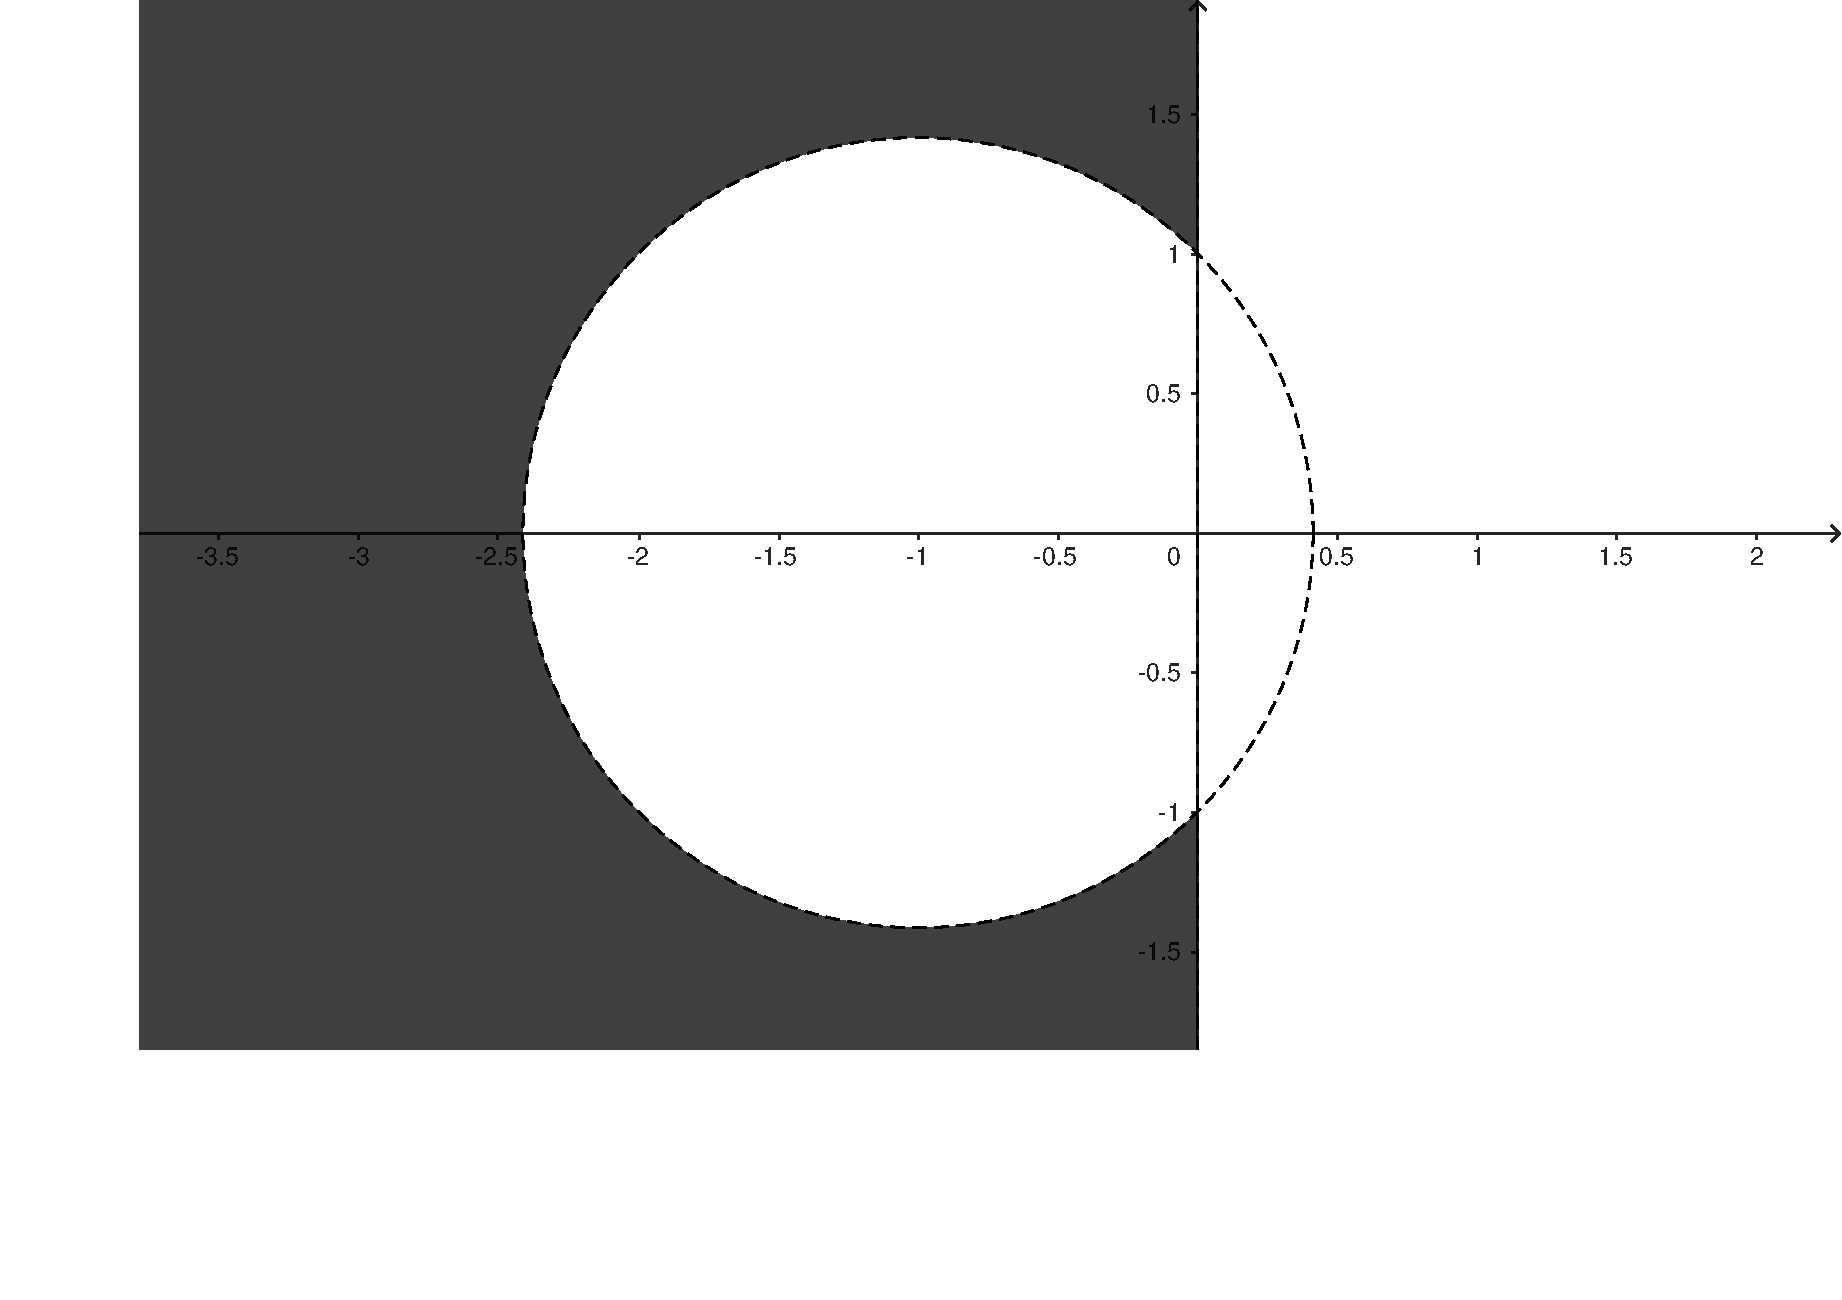
\includegraphics[width=.72\columnwidth]{figure/1.pdf}
\end{center}

\fbox{\parbox{\textwidth}{注释: 习题课已经讲过, \(\arg\) 和 \(\arctan\) 不等价. 很多人直接 \(0<\frac{-2x}{x^2+y^2-1}<1\), 算出两个区域的并.}}

\question{3}

\begin{center}
  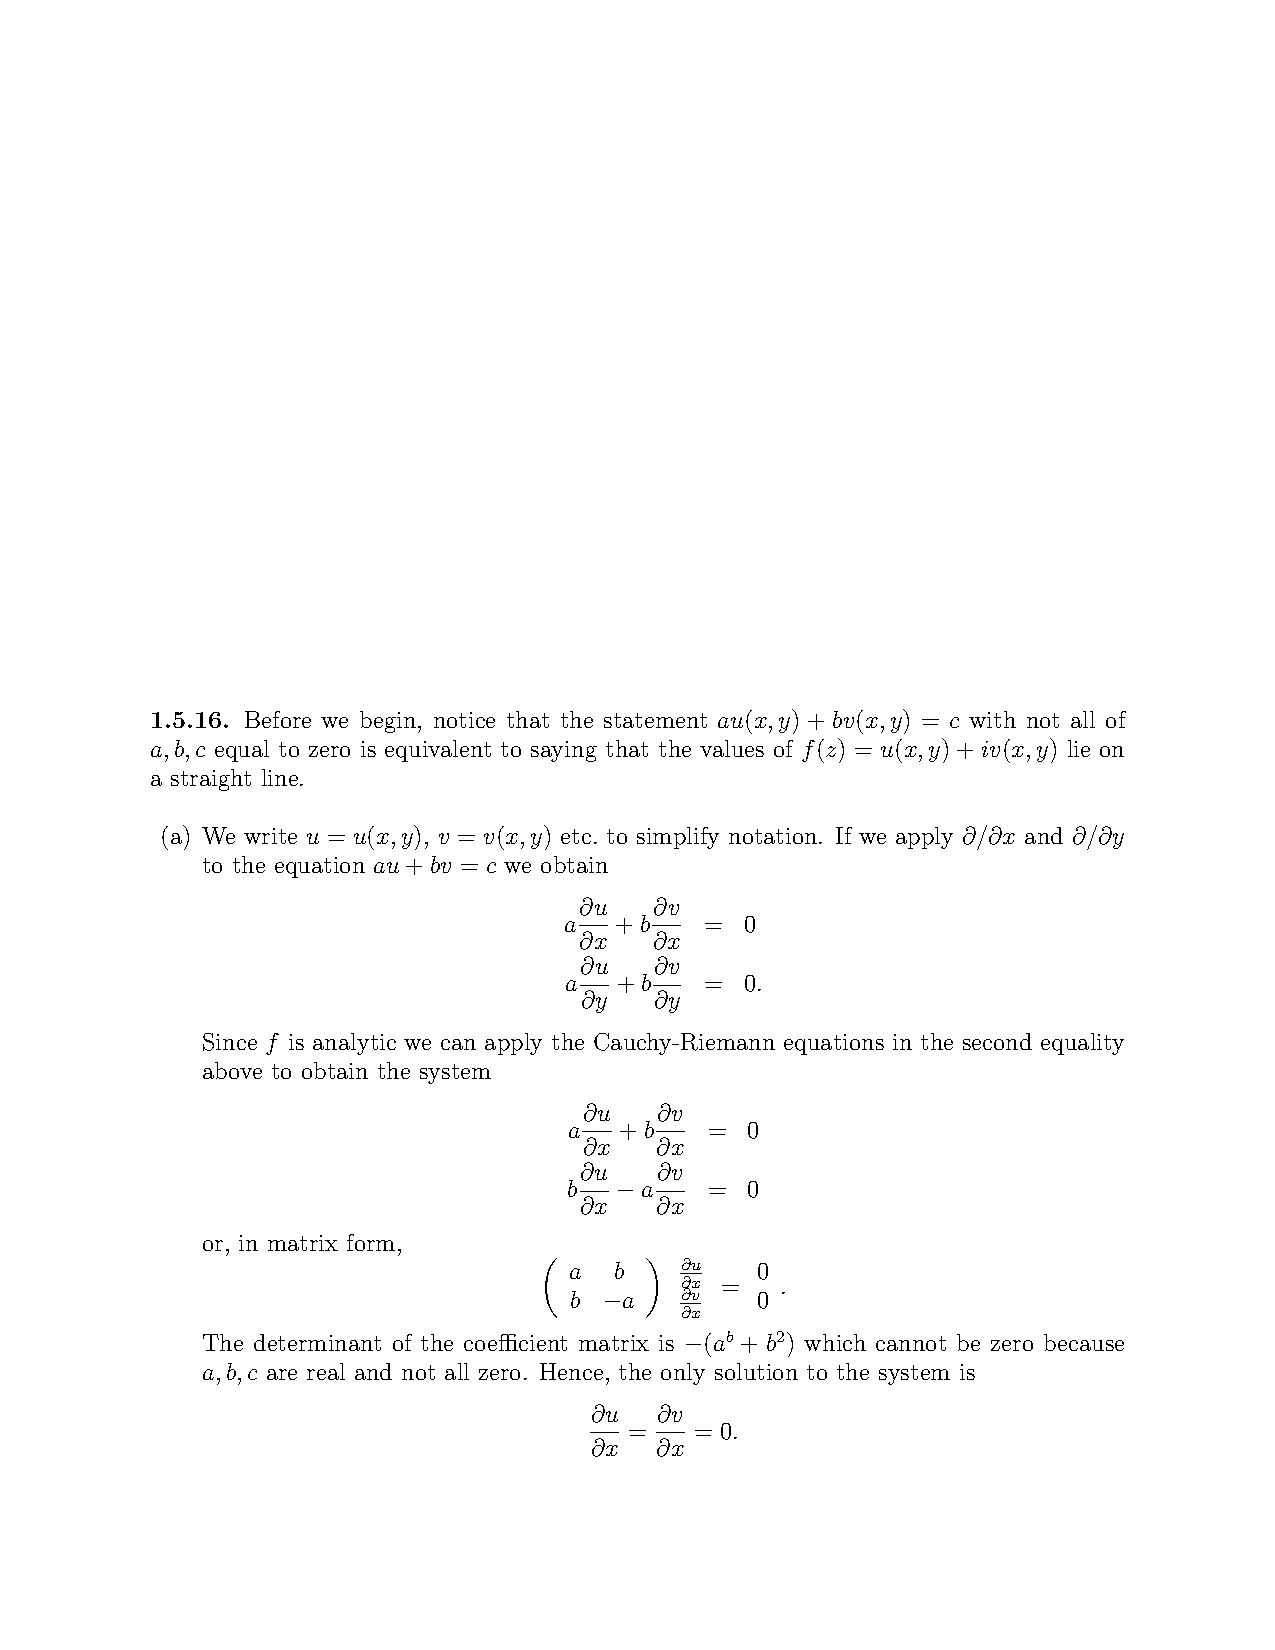
\includegraphics[page=1, width=\columnwidth]{figure/hw4_soln.pdf}
  \includegraphics[page=2, width=\columnwidth]{figure/hw4_soln.pdf}
\end{center}

Source: \href{http://ramanujan.math.trinity.edu/rdaileda/teach/m4364f07/hw4_soln.pdf}{link}.

\question{5}

首先验证 \(v(x, y)\) 是调和函数.

\(\frac{\partial v}{\partial x}=-\frac{\sqrt{-x+\sqrt{x^2+y^2}}}{2 \sqrt{x^2+y^2}},\)\hfill (2 分)

\(\frac{\partial v}{\partial y}=\frac{y}{2 \sqrt{x^2+y^2} \sqrt{-x+\sqrt{x^2+y^2}}},\)\hfill (4 分)

\(\frac{\partial^2 v}{\partial x^2}=-\frac{\left(-1+\frac{x}{\sqrt{x^2+y^2}}\right)^2}{4 \left(-x+\sqrt{x^2+y^2}\right)^{3/2}}+\frac{-\frac{x^2}{\left(x^2+y^2\right)^{3/2}}+\frac{1}{\sqrt{x^2+y^2}}}{2 \sqrt{-x+\sqrt{x^2+y^2}}},\)\hfill (5 分)

\(\frac{\partial^2 v}{\partial y^2}=-\frac{y^2}{4 \left(x^2+y^2\right) \left(-x+\sqrt{x^2+y^2}\right)^{3/2}}-\frac{y^2}{2 \left(x^2+y^2\right)^{3/2} \sqrt{-x+\sqrt{x^2+y^2}}}+\frac{1}{2 \sqrt{x^2+y^2} \sqrt{-x+\sqrt{x^2+y^2}}},\)\hfill (6 分)

\(\frac{\partial^2 v}{\partial x^2}+\frac{\partial^2 v}{\partial y^2}=0\), 故 \(v(x, y)\) 是调和函数.\hfill (9 分)

\(u(x,y)=\int_{(0,0)}^{(x,y)}\frac{\partial v}{\partial y}\,dx-\frac{\partial v}{\partial x}\,dy+C\).\hfill (10 分)

令 \(x, y\geq0\), 有
\begin{align*}
  u(x,y)&=\int_{(0,0)}^{(x,y)}\frac{y}{2 \sqrt{x^2+y^2} \sqrt{-x+\sqrt{x^2+y^2}}}\,dx+\frac{\sqrt{-x+\sqrt{x^2+y^2}}}{2 \sqrt{x^2+y^2}}\,dy+C\\
  &=\int_{(0,0)}^{(x,y)}\frac{\sqrt{x+\sqrt{x^2+y^2}}}{2 \sqrt{x^2+y^2}}\,dx+\frac{\sqrt{-x+\sqrt{x^2+y^2}}}{2 \sqrt{x^2+y^2}}\,dy+C\\
  &=\int_{0}^{x}\frac{\sqrt{x+\sqrt{x^2}}}{2 \sqrt{x^2}}\,dx+\int_{0}^{y}\frac{\sqrt{-x+\sqrt{x^2+y^2}}}{2 \sqrt{x^2+y^2}}\,dy+C\\
  &=\sqrt{2x}+\int_{0}^{y}\frac{\sqrt{-x+\sqrt{x^2+y^2}}}{2 \sqrt{x^2+y^2}}\,dy+C.
\end{align*}\hfill (12 分)

令 \(t=\sqrt{x^2+y^2}\), 则 \(y=\sqrt{t^2-x^2}, dy=\frac{t}{\sqrt{t^2-x^2}}\,dt\), 于是
\begin{align*}
  u(x,y)&=\sqrt{2x}+\int_{0}^{y}\frac{\sqrt{-x+\sqrt{x^2+y^2}}}{2 \sqrt{x^2+y^2}}\,dy+C\\
  &=\sqrt{2x}+\int_{x}^{\sqrt{x^2+y^2}}\frac{\sqrt{-x+t}}{2t}\frac{t}{\sqrt{t^2-x^2}}\,dt+C\\
  &=\sqrt{2x}+\int_{x}^{\sqrt{x^2+y^2}}\frac{1}{2\sqrt{t+x}}\,dt+C\\
  &=\sqrt{x+\sqrt{x^2+y^2}}+C.
\end{align*}\hfill (15 分)

因为 \(f(0)=0\), 故 \(C=0\).\hfill (16 分)

令 \(x=z\geq0, y=0\), 得 \(f(z)=u(x,y)+iv(x,y)=(2z)^{\frac{1}{2}}, z\in\mathbb{C}\).\hfill (20 分)

\fbox{\parbox{\textwidth}{注释: 习题课已经讲过, 这种题必须先验证调和函数, 最后结果也要用 \(z\) 表示. 我们先得到 \(f(z)\) 在实轴非负半轴处的函数表达式, 由唯一性定理即可推广至全复平面. 当然, 很多人这里积分没算对, 所有人都认为 \(y=0\) 时 \(\frac{y}{2 \sqrt{x^2+y^2} \sqrt{-x+\sqrt{x^2+y^2}}}=0\), 而没注意到此时分母也是 0. 如果不化简 \(\frac{y}{2 \sqrt{x^2+y^2} \sqrt{-x+\sqrt{x^2+y^2}}}\), 对于这种分子分母都为 0 的情形, 我们不能取 \(y=0\) 积分, 但可以取 \(y=1\) 积分, 此时积分路径变为 \((0,1)\rightarrow(x,1)\rightarrow(x,y)\). 或者, 也可以取积分路径 \((0,0)\rightarrow(0,y)\rightarrow(x,y)\). 另一个需要换元的积分算出来的寥寥无几, 为避免麻烦, 我们这里也可以用第 6 题的结论, 在极坐标下处理.

设 \(z=re^{i\theta}, \theta\in[0,2\pi)\), 则 \(v=\sqrt{r-r\cos\theta}=\sqrt{2r\sin^2\frac{\theta}{2}}=\sqrt{2r}\sin\frac{\theta}{2}\).

由\href{https://www.math.ucdavis.edu/~saito/courses/21C.w11/polar-lap.pdf}{极坐标系下的 Laplace 方程}, 我们可以验证 \(v(r, \theta)\) 是调和函数, 即满足:
\[\frac{\partial^2{v}}{\partial r^2}+\frac{1}{r}\frac{\partial v}{\partial r}+\frac{1}{r^2}\frac{\partial^2{v}}{\partial \theta^2}=0.\]

因为
\[\begin{cases}\frac{\partial v}{\partial r}=\frac{1}{\sqrt{2r}}\sin\frac{\theta}{2};\\\frac{\partial v}{\partial\theta}=\frac{\sqrt{2r}}{2}\cos\frac{\theta}{2}.\end{cases}\]
所以由第 6 题结论有
\[\begin{cases}\frac{\partial u}{\partial r}=\frac{1}{\sqrt{2r}}\cos\frac{\theta}{2};\\\frac{\partial u}{\partial\theta}=-\sqrt{\frac{r}{2}}\sin\frac{\theta}{2}.\end{cases}\]
于是
\begin{align*}
  u(r,\theta)&=\int_{(0,0)}^{(r,\theta)}\frac{\partial u}{\partial r}\,dr+\frac{\partial u}{\partial\theta}\,d\theta+C\\
  &=\int_{0}^{r}\frac{1}{\sqrt{2r}}\,dr-\int_{0}^{\theta}\sqrt{\frac{r}{2}}\sin\frac{\theta}{2}\,d\theta+C\\
  &=\sqrt{2r}-2\sqrt{\frac{r}{2}}(\cos\frac{\theta}{2}-1)+C\\
  &=\sqrt{2r}\cos\frac{\theta}{2}.
\end{align*}

因为 \(f(0)=0\), 故 \(C=0\).

令 \(r=z, \theta=0\), 得 \(f(z)=u(r,\theta)+iv(r,\theta)=(2z)^{\frac{1}{2}}, z\in\mathbb{C}\).

由此可见极坐标下处理更为简单. 若取积分路径为 \((0,0)\rightarrow(0,\theta)\rightarrow(r,\theta)\), 甚至只需计算一个积分.}}

\question{6}

设 \(\begin{cases}x=r\cos\theta;\\y=r\sin\theta.\end{cases}\)

则 \(\begin{bmatrix}
  x\\
  y
\end{bmatrix}=\begin{bmatrix}
  \frac{\partial x}{\partial r} & \frac{\partial x}{\partial\theta}\\
  \frac{\partial y}{\partial r} & \frac{\partial y}{\partial\theta}
\end{bmatrix}\begin{bmatrix}
  r\\
  \theta
\end{bmatrix}=\begin{bmatrix}
  \cos\theta & -r\sin\theta\\
  \sin\theta & r\cos\theta
\end{bmatrix}\begin{bmatrix}
  r\\
  \theta
\end{bmatrix}\).

由于\(\begin{bmatrix}
  \cos\theta & -r\sin\theta\\
  \sin\theta & r\cos\theta
\end{bmatrix}^{-1}=\begin{bmatrix}
  \cos\theta & sin\theta\\
  -\frac{\sin\theta}{r} & \frac{\cos\theta}{r}
\end{bmatrix}\),

故 \(\begin{bmatrix}
  r\\
  \theta
\end{bmatrix}=\begin{bmatrix}
  \cos\theta & sin\theta\\
  -\frac{\sin\theta}{r} & \frac{\cos\theta}{r}
\end{bmatrix}\begin{bmatrix}
  x\\
  y
\end{bmatrix}\).

那么 \(\begin{bmatrix}
  u\\
  v
\end{bmatrix}=\begin{bmatrix}
  \frac{\partial u}{\partial r} & \frac{\partial u}{\partial\theta}\\
  \frac{\partial v}{\partial r} & \frac{\partial v}{\partial\theta}
\end{bmatrix}\begin{bmatrix}
  r\\
  \theta
\end{bmatrix}=\begin{bmatrix}
  \frac{\partial u}{\partial r} & \frac{\partial u}{\partial\theta}\\
  \frac{\partial v}{\partial r} & \frac{\partial v}{\partial\theta}
\end{bmatrix}\begin{bmatrix}
  \cos\theta & sin\theta\\
  -\frac{\sin\theta}{r} & \frac{\cos\theta}{r}
\end{bmatrix}\begin{bmatrix}
  x\\
  y
\end{bmatrix}=\begin{bmatrix}
  \frac{\partial u}{\partial r}\cos\theta-\frac{\partial u}{\partial\theta}\frac{\sin\theta}{r} & \frac{\partial u}{\partial r}sin\theta+\frac{\partial u}{\partial\theta}\frac{\cos\theta}{r}\\
  \frac{\partial v}{\partial r}\cos\theta-\frac{\partial v}{\partial\theta}\frac{\sin\theta}{r} & \frac{\partial v}{\partial r}sin\theta+\frac{\partial v}{\partial\theta}\frac{\cos\theta}{r}
\end{bmatrix}\begin{bmatrix}
  x\\
  y
\end{bmatrix}\).

因此
\begin{gather}
  \frac{\partial u}{\partial r}\cos\theta-\frac{\partial u}{\partial\theta}\frac{\sin\theta}{r}=\frac{\partial v}{\partial r}sin\theta+\frac{\partial v}{\partial\theta}\frac{\cos\theta}{r}.\label{a}\\
  \frac{\partial u}{\partial r}sin\theta+\frac{\partial u}{\partial\theta}\frac{\cos\theta}{r}=-\frac{\partial v}{\partial r}\cos\theta-\frac{\partial v}{\partial\theta}\frac{\sin\theta}{r}.\label{b}
\end{gather}

\(\eqref{a}\cos\theta+\eqref{b}\sin\theta\) 得: \(\frac{\partial u}{\partial r}=\frac{1}{r}\frac{\partial v}{\partial\theta}\).

\(\eqref{a}\sin\theta-\eqref{b}\cos\theta\) 得: \(\frac{\partial v}{\partial r}=-\frac{1}{r}\frac{\partial v}{\partial\theta}\).

故极坐标下的柯西--黎曼方程是 \[\begin{cases}\frac{\partial u}{\partial r}=\frac{1}{r}\frac{\partial v}{\partial\theta};\\\frac{\partial v}{\partial r}=-\frac{1}{r}\frac{\partial u}{\partial\theta}.\end{cases}\]

\fbox{\parbox{\textwidth}{注释: 有一些同学貌似是提前知道答案, 利用\href{https://math.stackexchange.com/questions/1245754/cauchy-riemann-equations-in-polar-form}{配凑的方法}, 将 \(\frac{\partial u}{\partial r}, \frac{\partial u}{\partial\theta}\) 用 \(\frac{\partial u}{\partial x}, \frac{\partial u}{\partial y}\) 表示, 凑出最后的结论. 我们这里的思路是将 \(\frac{\partial u}{\partial x}, \frac{\partial u}{\partial y}\) 用 \(\frac{\partial u}{\partial r}, \frac{\partial u}{\partial\theta}\) 表示, 并代入直角坐标下的柯西--黎曼方程.}}

\end{document}